\section{Signal dimuon mass modeling}
\label{sig_model}

%
% Outline:
% - General Description of Signal Modeling
% - Choice of Pdfs
% - Procedure for Building/Fitting/Extracting Model Parameters
% - Normalization
%

%
% General Description
%
To be able to judge/draw conclusions about possible excess of events, due to the SM Higgs Boson, we ought to build a model aiming to explain the to be observed excess. Given we are looking for a bump-like structure near the Higgs Boson Mass, it is natural to model this excess via a composition of Gaussian functions. Each category and production process has been treated individually/separately and only depends on the Higgs Boson Mass and nuisance parameters to be described further. In the modeling we perform, we follow a similar approach that has previously been described in the Run~I $H\rightarrow\gamma\gamma$ analysis \cite{CMS-PAS-HIG-13-001,CMS_AN_2013-253}.

The Signal Model for the Higgs boson like signal accounts for both shape and normalization, fully parametric in $\mH$, and in the nuisance parameters described in section FIXME. %% ~\ref{xxx}{\bfseries}.

\begin{align}
   \label{eq:DoubleGaus}
   S(x,\mH, \theta) &= f \mathcal{N}_{1}(x, \mu_{1}, \sigma_{1}) + (1-f)  \mathcal{N}_{2}(x, \mu_{2}, \sigma_{2}) \\
   \label{eq:TripleGaus}
   S(x,\mH, \theta) &= f_{1} \mathcal{N}_{1}(x, \mu_{1}, \sigma_{1}) + (1-f_{1}) \left(f_{2} \mathcal{N}_{2}(x, \mu_{2}, \sigma_{2}) + (1-f_{2}) \mathcal{N}_{3}(x, \mu_{3}, \sigma_{3})\right)
\end{align}

where $\mathcal{N}(x,0,1)$ is a normal distribution, $\mu_i(\mH,\theta), \sigma_i(\mH,\theta)$ are respectively the mean and sigma of each gaussian, $x$ is the reconstructed invariant mass of the two muons (\mmm), and $\theta$ is the list of parametric nuisances.

%
% Choice of Pdfs
%
Both double eq~\ref{eq:DoubleGaus} and triple eq~\ref{eq:TripleGaus} Gaussian forms were tested.
The main reason for extending the form up to triple Gaussian (w.r.t. Run~I)
is to be able to pick up both the possible mass shift due to FSR and accomodate the broadening due to detector resolution effects.

%
% Procedure
%
For each category and each production process (ggH, qqH, WPlusH, WMinusH, ZH, ttH) , all of the signal parameters are derived by fitting a given model (Double eq~\ref{eq:DoubleGaus} or Triple eq~\ref{eq:TripleGaus} Gaus) to the dimuon invariant mass $\mmm$ spectrum obtained from the MC signal samples (described in FIXME %% section~\ref{sec:mc}
) being subject to the same event selection as data (section~\ref{event_sel}).
For the purpose of testing various Higgs Boson Mass hypotheses, three mass points ($\mH=120\,\gev$, $125\,\gev$, $130\,\gev$) were used, which allows us to interpolate in between and probe any mass in the range $[120, 130]\,\gev$.

The procedure to extract model parameters from the signal MC goes as following:
\begin{itemize}
    \item For a given category and production process
    \item Start with the invariant mass spectrum for $\mH$ of $120\,\gev$ and perform a binned maximum likelihood fit using initial default parameters.
    \item Proceed to next point in mass ($\mH$ of 125 GeV), by using the same fitted resolution ($\sigma_{i}$) from the previous fit ($\mH= 120\gev$) and shifted scale ($\mu_{i}$), by the mass difference, parameters as initial guesses.
        Perform the Maxlikelihood Fit and extract the parameters.
    \item Proceed to the $\mH$ of $130\,\gev$ and perform the same procedure as for $125\,GeV$.
    \item Each parameter $\mu_{i}, \sigma_{i}, f_{i}$ can be now interpolated across the mass points, using spline function.
    \item At this point, we have all the parameters ($\sigma_{i}$, $\mu_{i}$, $f_{i}$) be functions of $\mH$.
\end{itemize}

%% Fig.~\ref{sigmodel:gaus}
Figure~\ref{sigmodel:gaus} shows an example of fit with three gaussians on the left, an example of interpolation on the center, and an example of efficiency times acceptance on the right. All plots are available in FIXME.
%% Appendix~XXX.

 \begin{figure}[hbp]
     \centering
     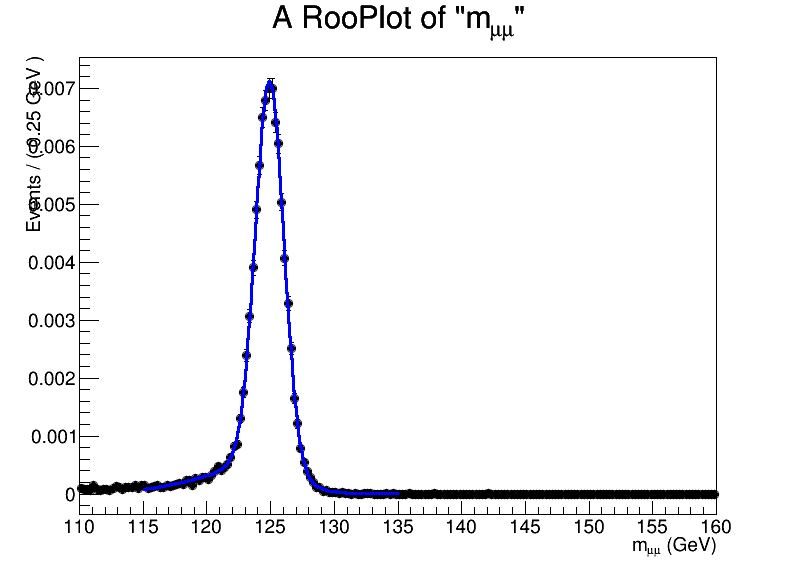
\includegraphics[width=0.3\textwidth]{figures/signal_model/baseline_all/signalFit__01JetsTightBB__125__GluGlu__TripleGaus__default.png}
     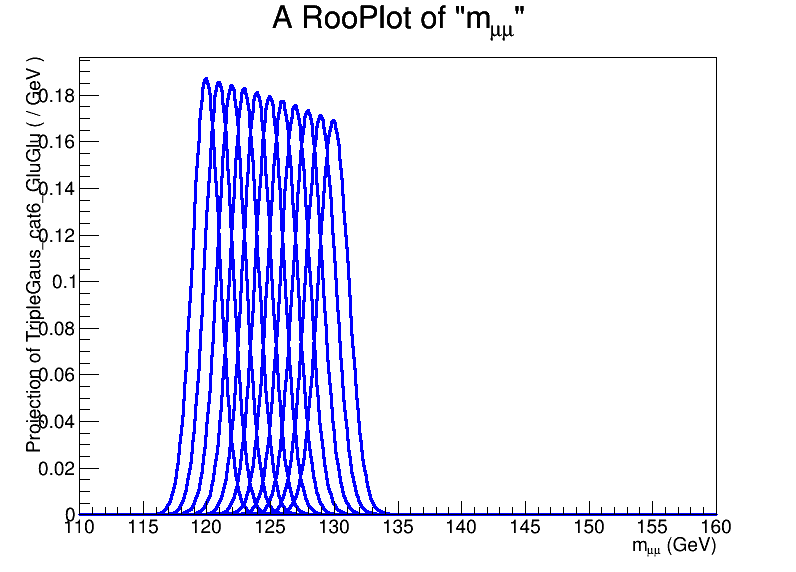
\includegraphics[width=0.3\textwidth]{figures/signal_model/baseline_all/signalFitInterpolationWithSpline__01JetsTightBB__GluGlu__TripleGaus__.png}
     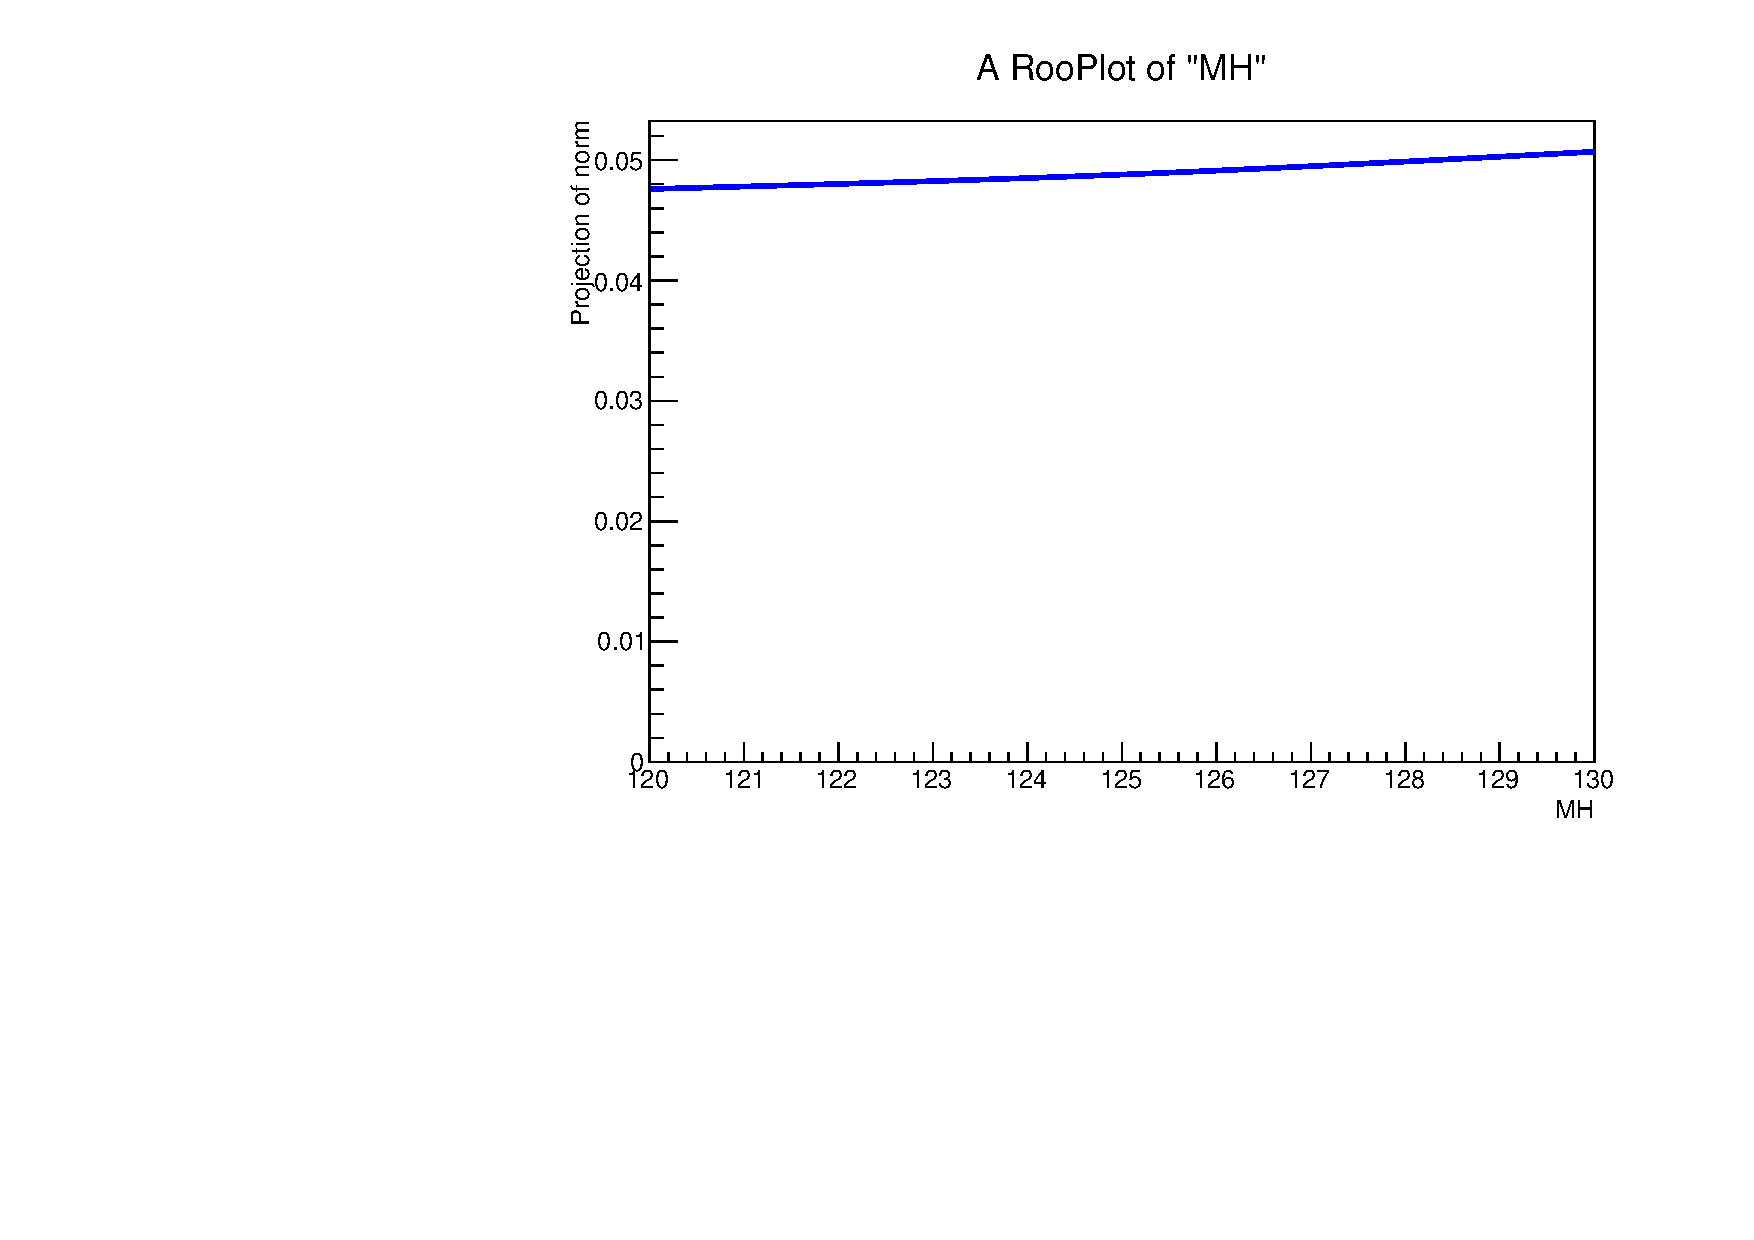
\includegraphics[width=0.3\textwidth]{figures/signal_model/baseline_all/effAcc_example.pdf}
     \caption{}
     \label{sigmodel:gaus}
 \end{figure}

%
% Normalization
%
The last missing piece for Signal Model building is the normalization.
Given a dimuon invariant mass distribution for a particular category for a particular production process,
the expected yields can be expressed as in equation~\ref{eq:expectedYield}.

\begin{align}
        %\label{eq:signalNormalization}
        %\text{Norm} = {\frac{\mathcal{L} \sigma \mathcal{B}(\Htomm)}{N_{gen}}} \\
        \label{eq:expectedYield}
        %\text{Yield} = {Norm \times \sum_{bins}^{} N_{i}}
        %\label{eq:efficienceAcceptance}
        \text{Yield} = \mathcal{L}\,\sigma(pp\rightarrow H)\, \mathcal{B}(\Htomm) \, \varepsilon A
\end{align}

The production cross sections ($\sigma(pp\rightarrow H+X)$) for each process and the branching ratio of the Higgs boson to decay into a muon pair ($\mathcal{B}(\Htomm)$) are taken from the Yellow~Report~4 \cite{YR4} as centrally provided in {\it combine} (see more on this in section~\ref{combine_tool}).

Effieciency times acceptance ($\varepsilon A$) is computed using the MC sample information as
\begin{align}
\varepsilon A = \frac{1}{N}\sum w_i r_{i} \text{sf}_i \mathbf{1}_\textup{catX}
\end{align}

where $w_i$ is the generator weight, $r_i$ is the ``pileup reiweighting'' factor used to match the truth pu distribution injected in the MC to the one measured in data,
$\text{sf}_i$ is the total scale factor associated to the event,  {\bf FIXME describe more or refer to something.}
$\mathbf{1}_\textup{catX}$ is the identity function on the classification ($1$ if the event is in the category, $0$ otherwise),
and $N$ is the total normalization factor at generator level $N=\sum w_i$, where the sums runs over the entire MC dataset.

%whose entries correspond to the weighted number of events ($\rm{N_{i}}$) per bin,
%the overall normalization is computed according to eq~\ref{eq:signalNormalization}.
%which we can rewrite in terms of efficience and acceptance as in eq~\ref{eq:efficienceAcceptance}.

%Eq~\ref{eq:efficienceAcceptance} demonstrates three different pieces that will come together later on in section~\ref{combine_tool} : Integrated Luminosity, Cross-Section ($\sigma$) and Branching Ratio, and $\epsilon A$.
%For the purpose of modeling, Integrated Luminosity is a single number that is measured centrally; $\epsilon A$ is the normalization we extract from SM Signal Samples and they come in as functions of $\rm{m_{H}}$. Finally, for Cross-Sections and Branching Ratios, which are also functions of $\rm{m_{H}}$, we use centrally provided values by Combine (see more on this in section~\ref{combine_tool}).

Figure~\ref{sigmodel:comp} shows the composition of the signal model in the different categories of the ``Bdt'' analysis, and the total efficiency times acceptance of the selection prior to categorization.

\begin{figure}[hbp]
    \centering
    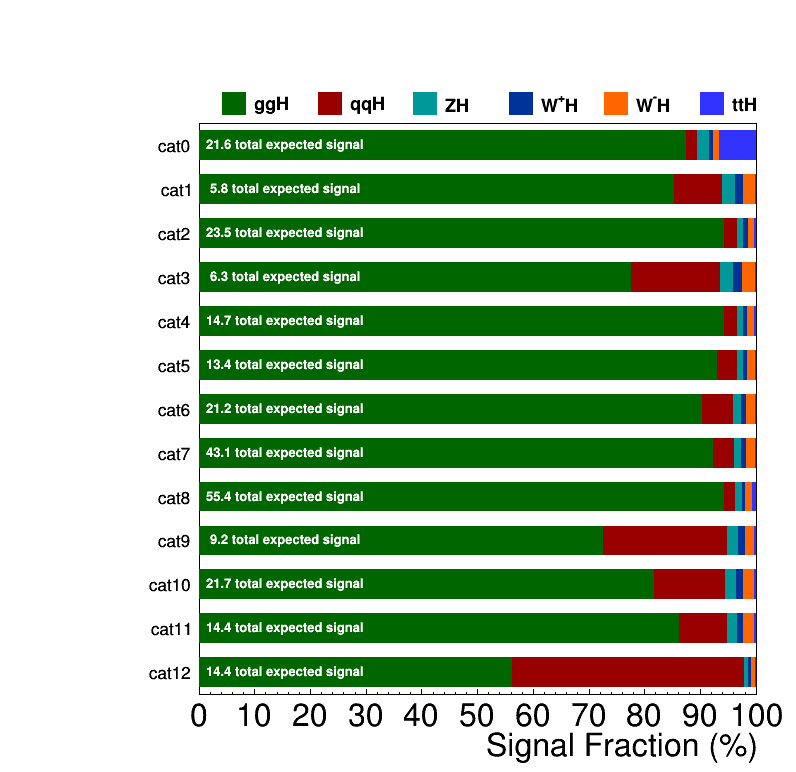
\includegraphics[width=0.49\textwidth]{figures/signal_model/signal_composition}
    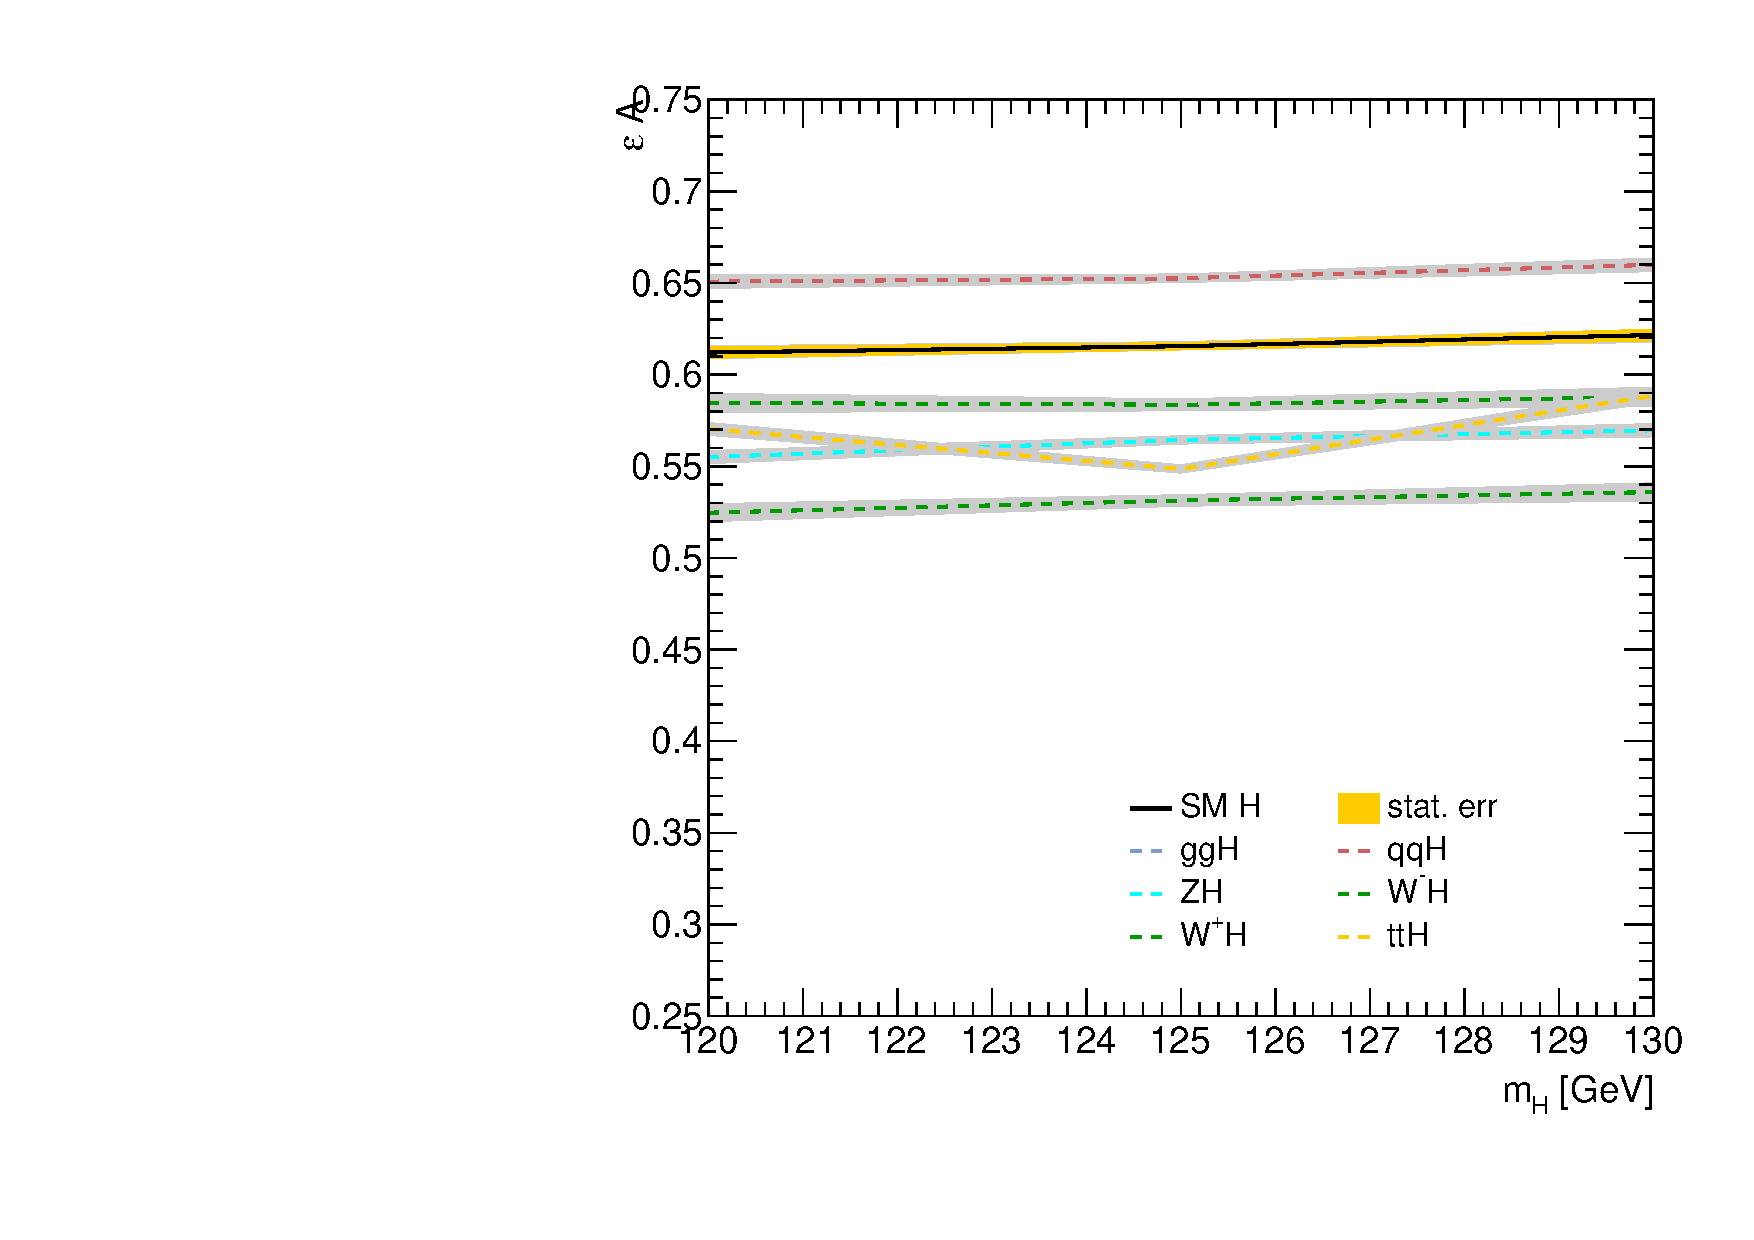
\includegraphics[width=0.49\textwidth]{figures/signal_model/effAcc}
    \caption{Left: Composition of the different categories of the ``Bdt'' analysis and expected yields of signal events.
    Right: Efficiency times acceptance of the total selection as function of \mH.}
    \label{sigmodel:comp}
\end{figure}

